%%%%%%%%%%%%%%%%%%%%%%%%%%%%%%%%%%%%%%%%%%%%%%%%%%%%%%%%%%%%%%%%%%%%%%%%%%%%%%
%%
%% A sample thesis using the cssethesis class
%%
%%%%%%%%%%%%%%%%%%%%%%%%%%%%%%%%%%%%%%%%%%%%%%%%%%%%%%%%%%%%%%%%%%%%%%%%%%%%%%
%%
%% Preamble
%%
% changed to onsided
\documentclass[a4paper,11pt,bcshonoursthesis,singlespace,oneside,thesisdraft,pdflatex]{cssethesis}
% * Include the option "pdflatex" above if you want to use pdflatex rather than
% standard latex to compile your document
% * Include the option "litreview" above if this is a literature review.
% * Include the option "nocoursecode" so that the numerical course code is
% suppressed after the course name.
% * Include the option "oneside" if you don't want formatting for two-sided
%   printing.
% * Include option "thesisdraft" to get a timestamp and "Draft" message in
%   the footer
% * Include option "thesispsdraft" to get a timestamp and "Draft" message in
%   the footer, along with a grey "DRAFT" in the margin. Note: this only
%   works with latex, not pdflatex

\usepackage{natbib} % Use the natbib bibliography and citation package
\usepackage{amsmath}
\usepackage{amssymb}
\usepackage{subfig}
\usepackage{tikz}
\usepackage{mwe}
\usepackage{listings}
\usetikzlibrary{arrows,automata}
\bibpunct{(}{)}{;}{a}{,}{,} % use more standard Harvard punctuation
\renewcommand{\cite}{\citep} % often a useful short-cut

% Definitions needed by the cssethesis class. See the documentation for
% others
\thesisauthor{Bradon Thomas Hall}
\thesisauthorlastname{Hall}
\thesisauthorpreviousdegrees{BSc, BCompSc} % Optional
%\thesisdepartment{Caulfield School of Information Technology} % Optional.
%                  Clayton School of Information Technology is the default
\thesisauthorstudentid{22051635} % Needed for litreview
\thesisauthoremail{bthal2\@@student.monash.edu.au} % Optional. Note that the @ is
											 % given as \@@. This is not
											 % necessary in normal LaTeX,
											 % but it is if you use the
											 % amsmath package - so why not
											 % get into the habit?
%\thesismonth{July} % Optional. Current month is used if this is not set
%\thesisyear{2002} % Optional. Current year is used if this is not set
\thesistitle{Simulated Evolution of Non-Regular Strategies for Repeated Games}
\thesissupervisor{Dr. Julian Garcia}
\thesissupervisoremail{julian.garcia\@@monash.edu.au} % Optional
%\thesisassocsupervisor{Dr. Fred Nurke} % Optional
%\thesisassocsupervisoremail{nurkef\@@csse.monash.edu.au} % Optional
%\thesisdedication{I luv youse all} % Optional

% start the document
\begin{document}

%%%%%%%%%%%%%%%%%%%%%%%%%%%%%%%%%%%%%%%%%%%%%%%%%%%%%%%%%%%%%%%%%%%%%%%%%%%%%%
%%
%% Front matter 
%%
\frontmatter					% start the thesis front matter.

\thesistitlepage				% Generate the title page.
\thesiscopyrightpage			% Generate the copyright page.
%\thesisdedicationpage			% Generate a dedication page (optional)
\tableofcontents				% Generate a table of contents.
\listoftables					% Generate a list of tables (optional).
\listoffigures					% Generate a list of figures (optional).

\begin{thesisabstract}			% generate the abstract page.
The evolution of strategies with varied conditions is investigated. 
Two mechanisms for cooperation are used; direct reciprocity and assortment. 
Strategies are represented by Deterministic Pushdown Automata. 
Strategies evolve in an evolutionary simulation. 
The cooperation that appears across the parameter space is recorded. 
I find varied levels of cooperation to previous simulations. 
The results in specified regions of the parameter space meet qualitative predictions in the literature.
A strategy not representable by past methods using Finite State Automata is found to evolve in the simulation. 
\end{thesisabstract}                 

\thesisdeclarationpage			% generate the declaration page (optional).

\begin{thesisacknowledgments}	% generate the acknowledgements page (optional).
I would like to thank my supervisor Julian Garcia, as well as my friends, family and colleagues for their support over this past year. In particular, thanks to Candace Nazareth and Melissa Hall for their support and helpful critique of my work over this year.
%I would like to thank everyone who helped to make this possible. It has
%been an incredible journey of self-discovery, and I love every last one of
%you\ldots
\end{thesisacknowledgments}   

%%%%%%%%%%%%%%%%%%%%%%%%%%%%%%%%%%%%%%%%%%%%%%%%%%%%%%%%%%%%%%%%%%%%%%%%%%%%%%
%%
%% Main matter 
%%
\mainmatter						% start the thesis body.

\chapter{Introduction}
\label{sec:intro}
In competitive environments, cooperation often emerges. 
Biology in particular is an example, with members of a population often working together to survive. 
I will consider cases where there is some benefit getting help, and some cost to giving help. 
For example, consider two predators sharing the food they capture in their separate hunts equally. 
The predator can choose to share half the spoils of their hunt with their partner (cooperate), or to deceive their partner and keep an uneven share. 
For simplicity, the deception is either full or not at all. 
There is a benefit to be had from mutual cooperation; assuming two equally adept hunters, a bad night hunting had by one will often be partially offset by the partners success. 
That is, risk is reduced, so there is a benefit of getting help. 
On the other hand, there is a cost to helping the partner -- part of the food is shared. A risk exists of deception by the partner, depriving the hunter of the benefit.  
How does cooperation emerge when individuals can benefit from exploiting others? 
 
We have some understanding of cooperation from experience and observation. 
If an encounter between two individuals is likely to re-occur, establishing cooperative behaviour is likely to pay off in the future. 
It might be worth taking the risk of being exploited now, to secure cooperation in the future if there is incentive to reciprocate. 
If reputation is part of the game, so other members of a population can observe how an individual behaves towards other members, cooperating could be a good idea in order to develop a reputation that you can be trusted. 
If success is measured by your genes passing on to a new generation, then it can be beneficial to cooperate with kin so they pass on the genes you share with them. 
These two ideas -- direct reciprocity and population structure (assortment) -- give mechanisms which could cause cooperation to be successful. 
Success is not measured only by relative performance in a single interaction. 
I will consider strategies that must interact in a changing environment. 
Some of the individuals they interact will occasionally change (mutate), and successful ones will reproduce -- it will be an evolutionary environment. 
A successful strategy must play the game well relative to others in the population to ensure its survival, but it must also perform well as that environment changes.

It is possible to investigate competition and cooperation mathematically -- Game Theory could be described as the mathematical study of competition and cooperation \citep{binmore2007playing}. 
Consider the case of repeated interactions; for a given scenario, how high does the likelihood of repeating an interaction have to be for cooperating to be the best strategy? 
In the case of cooperating with kin; how close should the relatives be for individuals to cooperate- should we cooperate fifth cousins, who share only a small number of genes? 

The literature that studies cooperation is broad. Direct reciprocity, where cooperation appears because the chance of encountering the same individual is high enough, has been well studied. 
Assortment, or population structure (such as a likelihood to interact with kin) has also been well studied. 
More recently, the interplay between reciprocity, structure, and resulting behaviour has been investigated \cite{van-veelen:PNAS:2012}. 
To study cooperation, a simple representation is used for the individuals that interact. One standard method is to use Finite State Automata. 
These machines have a collection of states and transitions between states. 
In a repeated game, the history is the series of moves that have occured so far in an interaction between two players. 
Based on the input -- the history of actions-- the transitions in an FSA are followed, moving states. 
How the individual behaves depends on what state it ends up on after following this history. 
If it ends on a state that is a final state, it cooperates. If it ends on a state that is not a final state, it defects. An example is shown in figure \ref{fig:fsa.tft.lang}. This strategy, called Tit-For-Tat (TFT) starts where the arrow indicates; which is an accepting state (indicated by two circles).

\begin{figure}
\center
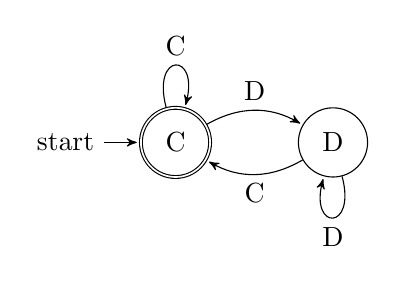
\begin{tikzpicture}[>=stealth',shorten >=1pt,auto,node distance=2cm]
\node[initial,state,accepting] (C)	{C};
\node[state] (D) [right of=C] {D};
\path[->] (D) edge [bend left] node {C} (C);
\path[->] (D) edge [loop below] node {D} (C);
\path[->] (C) edge [loop above] node {C} (C);
\path[->] (C) edge [bend left] node {D} (D);
\end{tikzpicture}
\caption{Tit-For-Tat as an FSA}
\label{fig:fsa.tft.lang}
\end{figure}

This representation does not cover all possible ways of choosing how to interact -- all strategies. In this thesis, I will examine the interplay between reciprocity and population structure, using a representation that examines a wider range of strategies than Finite State Automata do. 
%Finite State Automata define a class of strategies called Regular strategies. I will examine some strategies that Fininite State Automata cannot represent: Non-Regular Strategies (specifically, Deterministic Context-Free Strategies).
\section{Objectives and Research Questions}
%I have produced a simulation that can simulate the evolution of strategies in the Prisoner's Dilemma using a previously unexplored representation for those strategies. 
I aim to answer several questions by evolving strategies in simulation:
\begin{itemize}
\item How does enlarging the strategy space affect the level of cooperation that evolves? (Section \ref{sec:overall}). 
\item Do theoretical results (Section \ref{sec:pnas}) hold with the larger strategy space? (Section \ref{sec:regions}).
\item Do successful non-regular strategies evolve? (Section \ref{sec:dpdaresults})
\end{itemize}
 
By asking the last two questions in particular, I investigate the impact of the assumptions previous work has put on the capability of the strategies, and on what strategies can evolve. 

\section{Thesis Structure}
The remainder of this thesis will be structured as follows:
\begin{itemize}
\item Chapter \ref{chap:researchcontext}: Research Context, in which I discuss fundamentals of game theory and previous studies of the repeated Prisoner's Dilemma.
\item Chapter \ref{chap:researchmethods}: Research Methods, where I discuss the details of my simulation and how results are analysed
\item Chapter \ref{chap:results}: Results and Discussion, giving and discussing results of my work.
\item Chapter \ref{chap:conclusions}: Conclusion, where I summarise my work, and discuss future work.
\end{itemize}

\chapter{Research Context}
\label{chap:researchcontext}
In this chapter, I will discuss several aspects of Game Theory my work uses, as well as specific work into the Repeated Prisoner's Dilemma. 
Concepts from Game Theory will be discussed first, followed by as previous work into the simulated evolution of strategies for the repeated Prisoner's Dilemma. 
Finally, I will discuss work that investigates when reciprocity (repeating the game) is combined with assortment (population structure).
\section{Game Theory}
A game is a formalization of an interaction between two or more individuals who make choices. 
Depending on the choices made, each individual gains a payoff.  
I consider games where two players compete at once in particular, with any number of possible players who could be paired. 
Each player plays using a strategy, which we might represent explicitly, or we might simply state the payoff that the strategies gain against each other. 
Game Theory is the study of what strategies will be successful in a given scenario. 

The general approach in game theory is to consider a scenario, and simplify it. 
By doing this we examine the general dynamics of a situation. 
Each individual playing a game is assumed to try to maximize their personal payoff. 

For example; let us look circumstances where aggression or non-aggression are possible strategies. 
Two birds compete for a benefit; they fight for some food. 
A Hawk strategy escalates the fight. A Dove strategy fights with normal intensity against other Doves, avoiding injury, or retreats in response to escalation. 
A cost is assigned to escalating a fight (due to injury); call it $c$. 
A benefit is assigned to winning a fight, call it $b$. 
So, if an individual plays a Hawk strategy against a Hawk strategy, they have a 50/50 chance of winning since they are equivalent. Hawk-Hawk results in an expected payoff of $\frac{{b}-{c}}{2}$. 
When two Doves encounter each other, they don't get injured. 
They have a 50/50 chance of winning the non-escalated fight, so the expected payoff is $\frac{b}{2}$. 
A Dove retreats from a Hawk, avoiding injury but also losing any chance of getting the benefit. 
So, they get a payoff of $0$. A Hawk wins by default since the Dove retreats, avoids injury, and gets all the benefit; they recieve a payoff $b$. 

The payoff matrix for this scenario is given in Table \ref{table:payoffHD}.
\begin{table}[h]\centering
\captionsetup{justification=centering}
\begin{tabular}{|l|c|c|}
\hline
 & \bf{Hawk} & \bf{Dove}\\
\hline
Hawk & $\frac{{b}-{c}}{2}$, {$\boldsymbol{\frac{{b}-{c}}{2}}$} & $b$,$\boldsymbol{0}$\\
\hline
Dove & $0$,$\boldsymbol{b}$ & $\frac{b}{2}$,$\boldsymbol{\frac{b}{2}}$ \\
\hline
\end{tabular}
\caption{Payoff matrix for the Hawk-Dove game}
\label{table:payoffHD}
\end{table}

What is the best strategy to play? 
Assume that each individual has a strategy they are going to use -- they do not change their strategy. 
In a population of Doves, a lone Hawk will do well in comparison to the rest of the population, gaining the benefit (the food) without paying the cost (of injury). 
The rest of the population (Doves) gains either $\frac{b}{2}$ or $0$. 

In a population of almost entirely Hawks, how well a Dove does depends on the parameters. 
If the cost of injury is higher than benefit of winning the fight and getting the food, Hawks can be expected to get a negative payoff most of the time-- and so the lone Dove, with $0$ expected payoff may have the best expected payoff. In a population of 100 Hawks and 1 Dove, where each individual plays another individual randomly, a Hawk is expected to make $\frac{99}{100}\cdot\frac{b-c}{2}+\frac{1}{100}\cdot b$ and a Dove is expected to make $0$. If $c>b$, the Dove has the highest expected payoff. 

Existing literature in Game Theory allows us to analyse scenarios like these, and find what is the best strategy to play.
\subsection{Nash Equilibria}
The Nash Equilibria for a game are the strategies from which individuals have no incentive to switch. 
That is, they cannot get a higher payoff by choosing, on its own, to switch to a new strategy.  

A strategy $x$ is a Nash Equilibrium if it cannot increase its payoff playing any other strategy ($T$) in the set of possible strategies ($S$) by changing to another strategy ($x^\prime$) \citep[][ch. 1]{robert1992primer}:
\begin{equation}
\forall T \neq x, \{T,x\} \in S: \pi(x,T)\geq \pi(x^\prime,T)
\end{equation}
Where $\pi(A,B)$ is the payoff for $A$ when it plays against $B$. 
Alternatively stated, a Nash Equilibrium is found when a strategy is the best reply to itself. 
If the relation is greater than, it is a Strict Nash equilibrium. 
If it is greater than or equal to, it is a Nash equilibrium.

In the Hawk-Dove game for $c>b$, analysing the payoff for a Pure strategy (which always plays a stated strategy; in this one-shot version of the game, either Hawk or Dove) shows that neither is Nash. 
When playing against a Hawk (H), you would do better to switch to Dove and avoid the cost. 
When playing against a Dove (D), you would do better to switch to Hawk and gain the benefit $b$:
\begin{align*}
\pi(H,H)&\ngeq \pi(D,H)\\
\pi(D,D)&\ngeq \pi(H,D)
\end{align*}

Instead of playing with a single strategy, consider a scenario where two players probabilistically select an action. So, $p_1$ plays Hawk with probability $p$ and Dove with probability $p-1$. Strategies that make decisions probabilistically are Mixed Strategies. 
In this case, the expected payoff must be calculated based on probabilities of each move. 
Consider some strategy $p_1$ playing itself: 
\begin{align}
\label{eqn:probabilities}
\pi(p_1,p_1)&=\pi_{H,H}*p_{H,H}+\pi_{D,D}*p_{D,D}+\pi_{D,H}*p_{D,H}+\pi_{H,D}*p_{H,D}\\
\pi(p_1,p_1)&=\frac{b-c}{2}*p^2+\frac{b}{2}*(1-p)^2+0*(1-p)p+b*p(1-p) \nonumber
\end{align}
In a similar fashion, we can find the payoffs for all combinations of $p_1$ and $p_2$. 
In the example of the Hawk-Dove game, a Nash Equilibria does exist for mixed strategies \footnote{In this case, a strategy that has a p of $b/c$. See \cite{nowak2006evolutionary63}}. Pure strategies are the focus of this thesis.

\subsection{Evolutionary Stable Strategies}
Instead of a number of strategies competing, let's consider a population that changes over time. 
Players compete by playing a game. 
The payoff of that game results in a fitness, which determines the player's chance of reproducing. 
In addition, new members can enter the population as mutations to a players strategy can occur when they reproduce. 
In short, there will be random mutations and a selection condition (how well a player does in the population) -- it is an evolutionary environment. 

In an environment where strategies evolve, an extra condition must be added to see if a strategy will become most populous, and stay that way. 
In addition to not gaining a benefit from switching strategies in the immediate game, an Evolutionary Stable Strategy must survive in a population. 
For example, in the Hawk Dove game given earlier, a single Dove entering a population of Hawks can do quite well. 
That is, the population of individuals all playing Hawk have a lower fitness than a Dove invader. 
Its proportion in the population will grow; but Hawk gets a low payoff against itself. 
So, as its proportion rises its payoff falls. 
Will the population settle on some point? This will be discussed in Replicator Dynamics. 
For now, I discuss the circumstance under which a strategy will stay the most common strategy used in a population. 

For a strategy to be Evolutionarily Stable it must do better than any invader \citep[][ch. 2]{weibull1997evolutionary}. 
This is an extension to Nash:
\begin{align*}
\forall T \neq x, \{T,x\} \in S: \pi(x,T)&\geq \pi(x^\prime,T) \\ 
\text{if } \pi(x,T)=\pi(x^\prime, T)\text{ then }\pi(x, T) &> \pi(T,T)
\end{align*}
In this example, I will call $T$ an invader and $x$ a candidate for ESS. 
The non-strict Nash condition is used in this definition. 
The extra condition considers that any invader will at some point play itself. 
If the Nash condition is met, the invader does as well as the candidate against other strategies. 
If the second condition is not met and is instead equal (or less than), the invader performs equivalently to (or better than) each candidate. Each invader individual will have the same chance of reproducing as every candidate individual. 
The candidate does not prevent invasion. 

If the second condition is met, the invader cannot take over because sooner or later it plays itself, at which point it does worse than the candidate. 
The candidate is able to prevent invasion, and is an Evolutionary Stable Strategy. 

\subsection{Replicator Dynamics}
How strategies perform can be analysed with the Replicator equation \citep{hofbauer1998evolutionary}. 
The average fitness ($\phi(x)$) of a population ($x$, where $x_i$ is the proportion of strategy $i$ present) is found by summing total fitness of all unique members ($f_i(x)$, determined from payoffs) and multiplying by the proportion of each member. $N$ is the number of unique members:
\begin{equation}
\phi(x)=\sum_{i=1}^N x_i f_i(x)
\end{equation}
The rate of change of the number of $i$ in a population is dependent on the proportion of $i$ in the population, and the fitness in relation to the rest of the population:
\begin{equation}
\dot{x}_i=x_i [ f_i(x)-\phi(x)]
\end{equation}
Given a proportion of a population, the rate of change can be found. 
We can visualize how the strategies perform by plotting a phase diagram.  

Take the example of the Hawk-Dove game. Using two strategies, the diagram is a line with arrows indicating the dynamics. In this example, $b=2$ and $c=4$ (see Table \ref{table:hawkdove50}).

\begin{table}[h]\centering
\captionsetup{justification=centering}
\begin{tabular}{|l|c|c|c|}
\hline
 & \bf{Hawk} & \bf{Dove}\\
\hline
Hawk & -1, \bf{-1} & 2, \bf{0}\\
\hline
Dove & 0, \bf{2}  & 1, \bf{1} \\
\hline
\end{tabular}
\caption{Example Payoff matrix for the Hawk -- Dove game}
\label{table:hawkdove50}
\end{table}

\begin{figure}[h!]
\centering
\includegraphics[width=0.4\textwidth]{{hawkdove}.png}
\caption{Dynamics of Hawk -- Dove game with $b=2$ and $c=4$}
\label{fig:hawkdove}
\end{figure}

Figure \ref{fig:hawkdove} shows the diagram of the dynamics for the Hawk -- Dove game. 
When Hawks outnumber Doves, Doves are selected for. 
When Doves outnumber Hawks, Hawks are selected for. 
Therefore, the population settles on a mixture that includes both strategies. 
%An example with three strategies, giving a 2-d simplex, will be shown after I discuss repeating the Prisoner's Dilemma.

\section{The Prisoner's Dilemma}
\label{sec:prisoners}
The Prisoner's Dilemma is a simple model that has been widely used to study cooperation in repeated games \citep{Axelrod1997}. 
In the one-shot version of the Prisoner's Dilemma, cooperation is not the expected outcome. 
In this game, two players play a single game, choosing between two options; cooperate or defect. 
Players choose simultaneously, and have no information on the opponents choice before their own decision is made. 
If they both cooperate they receive a score of R (Reward for cooperation). 
If they both defect, they receive a score of P (Punishment for defection). 
If one player defects, and their opponent cooperates, the defector is rewarded with T (Temptation to defect). 
If a player cooperates, and their opponent defects, the cooperator receives a payoff of S (Sucker's punishment). 
The hierarchy of payoffs goes $T>R>P>S$. Table \ref{table:payoffs} shows the payoff matrix for the Prisoner's Dilemma. 
\begin{table}[h]\centering
\captionsetup{justification=centering}
\begin{tabular}{|l|c|c|}
\hline
 & \bf{Cooperate} & \bf{Defect}\\
\hline
Cooperate & R, \bf{R} & S, \bf{T}\\
\hline
Defect & T, \bf{S}  & P, \bf{P} \\
\hline
\end{tabular}
\caption{Payoff matrix for the Prisoner's Dilemma}
\label{table:payoffs}
\end{table}

Assuming both players are aware of the payoff table and both players act to maximise their personal payoff, defection is the strategy both players choose. 
If the opponent defects, the best move is to defect too to avoid paying the cost. 
If the opponent cooperates, the best move is to defect to avoid the cost, and gain the benefit. 
That is, the player can only lessen the payoff by cooperating -- mutual defection is a Nash equilibrium. 
The dilemma arises from the fact that mutual cooperation (R) would be a better total payoff for the players than the equilibrium of mutual defection (P). 
This game captures the essence of the problem of cooperation.
%TOTO: Rename ?
\subsection{Repetition: Stuck in the Dilemma}
When the Prisoner's Dilemma is played multiple times, all parties defecting is no longer the only successful strategy. 
For the repeated Prisoner's Dilemma, the number of games played is not known by players in advance. 
If both players knew how many rounds were to be played, the best move in the last round is defection. 
The same logic causes the second last round to be a defection, and the problem reduces to the Nash equilibrium of the one-shot version. 
A way to accomplish having an unknown number of rounds is to make future encounters probabilistic, the chance of another encounter between two players is given by the continuation probability $\delta$.

\citet{garcia:PLoSOne:2012} calculate the payoff for strategy A from repeated games with strategy B as
\begin{equation}
\label{eqn:repeatedPayoff}
\Pi_{AB}=(1-\delta)\sum^{\infty}_{t=0} \delta^i\pi^i_{AB}
\end{equation}
where $\delta$ is the continuation probability, and $\pi^i$ is the payoff from the $i$th round. 
The sum represents the diminishing likelihood of another game between the two players. 
The term $(1-\delta)$ is for convenience, normalising the payoffs.
 
Two simple strategies possible in the repeated version are Tit-For-Tat (TFT) and Suspicious Tit-For-Tat (STFT). 
Tit-For-Tat starts cooperating on the first round, then reciprocates the opponents last move. 
Suspicious Tit-For-Tat defects on the first round, then reciprocates the opponents last move. 
If ALLC plays TFT, in all rounds they are cooperative.  
If TFT plays STFT they alternate defect and cooperate (Figure \ref{table:reciprocity}). 
This behaviour highlights an example of a mechanism for the evolution of cooperation; direct reciprocity. 

\begin{figure}[h]
\centering
\captionsetup{justification=centering}
\begin{tabular}{|l|c|c|c|c|}
\hline
TFT & C & D & D&...\\
\hline
ALLD & D & D &D&...\\
\hline
\end{tabular}\hfill
\begin{tabular}{|l|c|c|c|c|c|}
\hline
TFT & C & D&C&...\\
\hline
STFT & D & C&D&...\\
\hline
\end{tabular}\hfill
\begin{tabular}{|l|c|c|c|c|c|}
\hline
ALLC & C & C&C&...\\
\hline
STFT & D & C&C&...\\
\hline
\end{tabular}\hfill
\caption{Simple strategies playing the Prisoner's Dilemma}
\label{table:reciprocity}
\end{figure}

Previously, the Replicator Equation was discussed. 
What does the resulting simplex look like when ALLC, TFT and ALLD are compared? 
For simplicity, I consider a case when the game is played 10 times. 
The result is pictured in Figure \ref{fig:allcalldtft}. 
Payoffs were calculated manually, and the dynamics graphed using Dynamo \citep{dynamo}.

\begin{figure}[h!]
\center
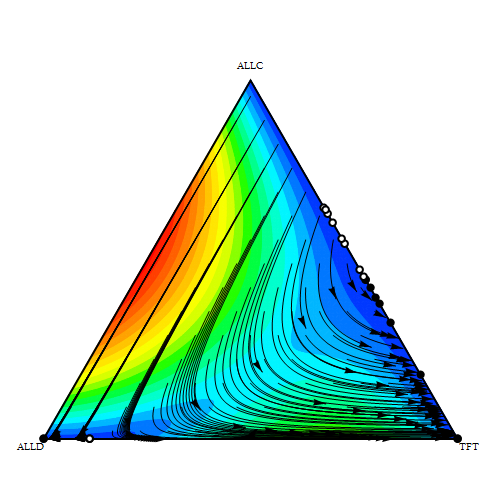
\includegraphics[width=0.6\textwidth]{allcalldtft}
\caption{Dynamics of ALLC, ALLD and TFT with a game of length 10}
\label{fig:allcalldtft}
\end{figure}
 
These diagrams visualize the resulting dynamics -- what strategies will be selected for in a given population \citep{imhof:PNAS:2005}. 
For example, a small number of ALLD players can quickly take over a population of ALLC players, since ALLD gains a better payoff. The arrows give the direction of selection, and the color indicates the speed. A population of ALLC moves towards ALLD. 
TFT and ALLC are neutral -- so drift can occur in either direction. 
When a mixture of strategies exists, in the interior of the simplex, TFT is favoured. 
In a full ALLD environment, TFT cannot invade; the ALLD corner has a black dot, indicating it is asymptotically stable. 
Likewise for ALLD invading TFT directly; however if the population drifts to ALLC, ALLD will invade. 

\subsection{Assortment}
Another mechanism to allow evolution of cooperative behaviour is to add structure to the population. 
This also better reflects many situations that can be modelled with evolutionary simulations \citep{eshel:PNAS:1982}. 
In nature, interaction between members of a population is not likely to be randomly distributed; interaction is more likely between kin, or social peers. 
Structure can be added by changing the probability of interactions- a subset of a population is more likely to interact with that subset. 

The expected payoff for a strategy in both a structured and unstructured environment can be found analytically \citep{van-veelen:PNAS:2012}. 
Consider a strategy space consisting of only always defect and always cooperate (ALLD, ALLC). 
The potential payoff ($\Pi$) for each strategy can be calculated by the probability of meeting an ALLC opponent times the payoff in that instance plus the probability of meeting an ALLD opponent times the payoff in that instance. Where $N_{TYPE}$ is the number of a type in a population, and $N_{TOTAL}$ is the total population size ($N_{TOTAL}=N_{ALLC}+ N_{ALLD}$), the payoffs are:
\begin{align*}
\Pi_{ALLC}&=\frac{N_{ALLC}-1}{N_{TOTAL}-1} \cdot (R) + \frac{N_{ALLD}}{N_{TOTAL}-1}\cdot ({S})\\
\Pi_{ALLD}&=\frac{N_{ALLC}}{N_{TOTAL}-1} \cdot (T) + \frac{N_{ALLD}-1}{N_{TOTAL}-1}\cdot ({P})
\end{align*}

In the case of an unstructured population, since $T>R$ and $P>S$, $\Pi_D$ always has a better payoff (excluding the case when $N_{ALLD}=0$). 
Instead take the case when the population is structured, and chance of meeting an alike player is r (structure parameter):
\begin{align*}
\Pi^{(r)}_{ALLC}&=(1-r)\Pi_{ALLC}+ rR\\
\Pi^{(r)}_{ALLD}&=(1-r)\Pi_{ALLD}+ rP
\end{align*}

Sufficiently higher probability of meeting an alike player allows cooperativity to have the greater payoff. 
Trivially, if probability of meeting like is 1, $\Pi^{(S)}_{ALLC}=R>\Pi^{(S)}_{ALLD}=P$, so cooperation has higher fitness.  
Substitution of values shows it holds for other cases. 
For example, if T=3, R=2, P=1, S=0, and the population is 50 ALLC and 50 ALLD:
\begin{align*}
\Pi^{(S)}_{ALLC}&=(1-r)(2\frac{49}{99})+r*2=\frac{98}{99}+\frac{198}{99}r-\frac{98}{99}r=\frac{1}{99}(98+100r)\\
\Pi^{(S)}_{ALLD}&=(1-r)(3*\frac{50}{99} + \frac{49}{99})+ r*1=\frac{199}{99}-\frac{199}{99}r+\frac{99}{99}r=\frac{1}{99}(199-100r)
\end{align*}
So ALLC has higher fitness if $r>101/200$. These cases demonstrate that structure can benefit cooperation. 
\section{Representing Strategies}
Previously discussed methods of analysing strategies for the repeated Prisoner's Dilemma have some limitations. 
To model with the replicator equation and plot a phase diagram to see the dynamics, a very small subset of strategies must be chosen. 
If we know or can guess what strategies will be important, this might be an effective tool. 
One way to find what strategies will be important is through simulating an evolutionary environment. 

Instead of picking the strategy, we pick a representation. 
A strategy takes a History $\mathcal{H}$ of previous moves in an interaction, and maps it to the action $\mathcal{A}$ the strategy decides to use:
\begin{equation}
f: \mathcal{H} \rightarrow \mathcal{A}
\end{equation}
The representation will be able to represent a subset of all possible strategies $f$ for the repeated Prisoner's Dilemma. 
In the case of the simulation presented in this thesis, $\mathcal{H}$ contains previous moves of an opponent -- so a sequence of $\{C,D\}$. 
If instead the full history is recorded -- a combination of both what the opponent and the strategy itself did-- a sequence of pairs of $\{C,D\}$ or a sequence of results $\{R,T,S,P\}$ would be recorded. \citet{axelrod1987evolution} and \citet{fogel1993evolving} are two examples of work using this 'full-memory' representation that will be discussed in \ref{sec:relatedWork}.
%MARKME
In addition to the method to map from a History to an Action, a mutation scheme is also needed; to take an existing strategy and create a new one. 
This will allow the creation of strategies, without the researcher needing to design or pick any \citep{koza}. 

Previous work has primarily used a Finite State Automata model for strategies. 
An even simpler representation is that of the Lookup Table. 
I will discuss both these methods in the next section. 
\subsection{Lookup Tables}
\label{sec:mutation}
One approach to representing strategies is to have a list of possible histories, and how to respond to that history. This is called a Lookup Table. 

For example, consider a representation that consists of a binary string of length 3 \citep{garcia:PLoSOne:2012}. A $0$ represents a choice to cooperate, a $1$ represents a choice to defect. 
The first digit represents the move performed in the initial game, when no history exists between two players. 
The next two digits determine the choice made, based on the previous choice made by the opponent and discarding all previous history. 
The second digit in the three digit string describes what the strategy does in response to a cooperation. 
The final digit describes what the strategy does in response to a defection. 
Table \ref{table:binaryStrategy} describes some of the possible strategies, selected for being simple and common (ALLD, ALLC), a successful strategy in previous studies (TFT), or as an example of a strategy that is nasty (defects at first), but will cooperate (STFT).

\begin{table}[h]
\centering
\captionsetup{justification=centering}
\begin{tabular}{|l|c|c|}
\hline
 Strategy & Description & Representation\\
\hline
ALLD & Always Defect & 111\\
\hline
ALLC & Always Cooperate & 000\\
\hline
TFT & Cooperate, then repeat opponents last move & 001\\
\hline
STFT & Defect, then repeat opponents last move & 101\\
\hline
\end{tabular}
\caption{Binary String representation for strategies}
\label{table:binaryStrategy}
\end{table}

The length 3 binary string representation can explore a set of $2^3=8$ strategies. Increasing the size of the string can allow for longer histories. 
If all except the last two moves are discarded, decisions are made based on the last two moves. 
With this representation $2^7=32$ strategies can be represented. 

Part of what makes this a good example representation is that it allows for several example mutation schemes. 
We could vary the strategies by flipping a bit in the string that represents the strategy. 
Other examples could include multiple flips, or inverting the entire string. 
Crossover could be used; selecting a new strategy with parts from the lookup table of 2 parents.

Alternatively, we could use a `mutation kernel' that indexes all strategies possible. 
For a 3-bit lookup table, this would require an 8x8 matrix, that gives the probability of mutating from any of the 8 states to any other of the 8 states. 
The mutation kernel could assume uniform mutations; that any one state is reachable from any other state in a single mutation. 
Each term in the matrix could also have some other justification; it could be based on the number bit flips to get from one strategy to another. 
\citet{garcia:PLoSOne:2012} showed the results from uniform or bitwise kernels differed; cooperative strategies were less common with the bitwise kernel. 

%Knowing that mutation schemes matter, how should we go about picking one?
%If we are simulating some biological process, we could base our mutation scheme on biological %factors. 
%The approach in this thesis is to design a scheme with minimal mutations, that can explore the entire strategy space representable by the computational model used. 

\subsection{Finite State Automata}
\label{sec:fsa}
Another common representation is Finite State Automata. 
A Finite State Automaton consists of a set of states, a set of transitions from state to state, and each state can be marked as an accepting state. 
Based on the history between two players in the current interaction, the transitions are followed until the complete history has been read. 
If the state the automaton ends up on is an accepting state, the individual represented by that automaton Cooperates, if not, they Defect. 

More formally, an FSA consists of:\\
1. A finite, set of states $S \neq  \emptyset$\\
2. An input alphabet, $\Sigma \neq  \emptyset$\\
3. A transition function $\delta : S \times \Sigma \rightarrow S$\\
4. A set of final/accepting states $F \subseteq S$ \\
5. The initial state $q_0 \in S$

An example is shown in Figure \ref{fig:fsa.tft.lang2}. 
In this example, there are 2 states; $S=\{D,C\}$. 
The set of accepting states contains one state; $F=\{C\}$. 
The input alphabet is $\Sigma=\{C,D\}$ and $C$ is the initial state. 
There are four transitions; $C$ to $C$ when C is read, $D$ to $C$ when C is read, $C$ to $D$ when D is read, and $D$ to $D$ when $D$ is read.

\begin{figure}[h]
\center
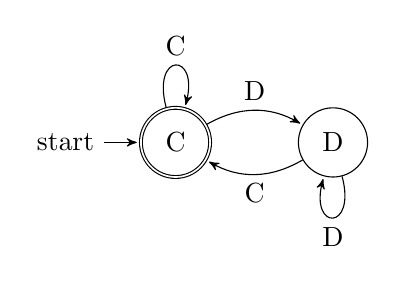
\begin{tikzpicture}[>=stealth',shorten >=1pt,auto,node distance=2cm]
\node[initial,state,accepting] (C)	{C};
\node[state] (D) [right of=C] {D};
\path[->] (D) edge [bend left] node {C} (C);
\path[->] (D) edge [loop below] node {D} (C);
\path[->] (C) edge [loop above] node {C} (C);
\path[->] (C) edge [bend left] node {D} (D);
\end{tikzpicture}
\caption{Tit-For-Tat as an FSA}
\label{fig:fsa.tft.lang2}
\end{figure}

It is common that the transition function $\delta$ is a total function in Prisoner's Dilemma's -- for every possible input (of a symbol from the input alphabet $\Sigma$) at any state a transition exists. 
This is not a strict requirement; if no valid transition exists for an input the input is not in the language, but the FSA is still valid (and will defect, since the input is not in the language represented by the FSA). 

FSA with multiple valid transitions for some input are Non-Deterministic FSA. 
FSA with only one valid transition for any input are Deterministic FSA. 
For every Non-Deterministic FSA, there is a Deterministic FSA that produces the same result for any valid input, equivalently; the two types of FSA can represent the same classes of languages/strategies \citep[][pp 35 -- 63]{Sipser2006}. 

A number of mutation schemes for Finite State Automata could also be used. 
These could involve adding states, deleting states, changing a transition, changing if a state is accepting, and changing the initial state. 
This graph based view is used in \cite{van-veelen:PNAS:2012}. 

Alternatively, we could set the number of states to a constant or upper limit and represent the FSA by a string; for example a 4 state machine could be given as in Table \ref{table:fsa4state}:
\begin{figure}[h]
\center
\begin{tabular}{|c|c|c|c|c|c|c|c|}
\hline
0C & 0D & 1C&1D&2C&2D&3C&3D\\
\hline
00 & 01 & 00&01&10&10&11&11\\
\hline
\end{tabular}\hfill
\caption{String representation for a 4 state FSA}
\label{table:fsa4state}
\end{figure}
The FSA given in \ref{table:fsa4state} is the equivalent of TFT, given earlier. 
Each column gives what to do if you are at a certain state, and read a certain input. 
So, at state 0 you transfer to state 0 (00) if you read C. 
You transfer to state 1 (01) if you read D. 
So, an FSA can be represented by a string (in this case 0001000110101111) or number. 
Mutation schemes discussed in Lookup Tables can also be applied to FSA. 

Variants on these representations are used in the work discussed.
\section{Related Work}
\label{sec:relatedWork}
Related simulation work focuses mostly on direct reciprocity; repeating the game being the basis for cooperation to evolve. 
I will discuss seminal work into strategies for the Prisoner's Dilemma, giving examples of different approaches in the literature. Finally, in Section \ref{sec:pnas} I will discuss the work I have extended.
\subsection{Axelrod's Tournaments}
\citet{axelrod:Science:1981} investigated the behaviour of strategies using computer tournaments, with the repeated Prisoner's Dilemma played between strategies submitted by people to the tournaments. 
This study compared fitness (payoff of games) of submitted strategies playing each other. 
Strategies play each other probabilistically; the game is not a fixed size, instead a continuation probability determines if they continue to play. Out of the 14 submitted strategies, Tit-For-Tat (TFT) performed best. 
Introduced in Section \ref{sec:intro}, this is a simple strategy that reciprocates the other player's behaviour, after initially cooperating. 
Initially it cooperates, then it repeats the other player's last move. 
When playing a strategy that always cooperates (ALLC), it performs identical to ALLC. 
When playing a strategy that always defects (ALLD), it loses on the first turn, then performs identical to ALLD -- given a long enough number of games played, the strategies have similar payoffs. 

Axelrod and Hamilton identified three criteria to determine if a strategy can be successful. The strategy must be robust- it must perform fairly well against a wide variety of strategies. TFT does so, including against the a population composed of the simple ALLC and ALLD examples, but only if there is a sufficient chance of the game repeating. Secondly, the strategy must be stable- a mutant strategy must not be able to invade in the event the strategy becomes established. For example, ALLC is not stable against ALLD. 
A single ALLD in a population of ALLC will gain better payoffs (fitness) and invade. 
Lastly, the strategy must be initially viable -- it must be able to gain a foothold. 

The Tournaments provide insight into the role Direct Reciprocity can play as a mechanism for the success of cooperation. 
A desirable extension is to allow evolution of the strategies, rather than just allowing the example strategies to compete. 
From the outcome of the tournaments one might initially suspect Tit-For-Tat might emerge and always dominate. However, \citet{boyd1987no} showed this might not be the case; Tit-For-Tat is not (and indeed no strategy is) evolutionary stable in the repeated dilemma game \citep{boyd1987no}. 
%van2010and
%Axelrod also let the players compete in an evolutionary environment. 
%*Axelrod population vs population 1987 might be worth it here*

A limitation of this method is the requirement for strategies to be designed rather than evolved. 
Naturally, this limits the strategies investigated to those the submitters or researchers could design.

\subsection{Evolving Strategies in Simulations}
\label{sec:axelrodEvolving}
\citet{axelrod1987evolution} used a simple Genetic Algorithm approach to study the evolution of strategies for the Prisoner's Dilemma \citep{back1997handbook}. A half-memory approach is one in which the opponent's sequence of Cooperate (C) or Defect (D) moves are remembered. A full memory approach remembers its own moves, or equivalently the results (both C is the same as Reward, R, both D is the same as Punish, P, etc). A string of \{C,D\} represents each strategy. A Full-Memory approach was used in \citet{axelrod1987evolution}. 

Based on previous moves, a location in that string is looked up, and states the next move to perform. 
The first 6 bits determines the initial strategy, then there is not a history of 3 moves. 
It gives a `history' to base decisions on, when no actual history is available. 
6 bits are required since both the opponents and their own moves need to be encoded. 
To encode the strategy, 64 bits are used. Three moves are remembered, with 4 possibilities- so $4^3$. 
A total of 70 bits were used by Axelrod's simulation, allowing for moves to be determined based on the last 3 results. That is, it is a full-memory simulation of length 3. 
This allows for any of $2^{70}$ different strategies to appear- analysis using a matrix of payoff of every strategy against every other strategy would be a square matrix with $2^{70}$ elements on each side. 
This is why explicit analysis selects notable examples from the population, and demonstrates why simulation will be useful. 

Strategies are generated in a population, and then they compete with 8 strategies from the original tournaments to determine their fitness. A new population is determined by reproducing from the population, with fitness determining what strategies reproduce. They then compete with the 8 representatives again. 
Reproduction involves a small chance of random mutation, and a crossover from each parent. 
The string representing the strategy is the chromosome, and the new child is produced from parts of each parent's chromosome. A population of 20 strategies competed in games 151 moves long, competing with 8 other members of the population in each round, for 50 generations. 
Technology of the time limited the size of simulations; today we have the luxury of being able to throw far more computing power at the problem, allowing for much longer (and with larger population) simulations. 
The initial population was random. The strategies that evolved mostly resembled Tit-For-Tat, and Axelrod identified general patterns for strategies. They continued cooperating after mutual cooperation had been established, they responded to opponent defection with defection, they returned to cooperation after it was restored by the opponent following a defection, and when stuck in a pattern of mutual defection they do not attempt to escape and allow themselves to be exploited. 

Strategies that performed better than Tit-For-Tat did emerge. These developed ways to exploit one of the 8 representatives, having a higher fitness against that, at a cost of a lower fitness against some of the other 8 representatives. If the net result is a gain over Tit-For-Tat, the strategy performs better. 
This only applies to the environment of this simulation. 
In an environment where the competing strategies is not fixed, for example when the competition is picked from the population, those exploited strategies might be expected to die off and remove the advantage the exploiter gains. 

Axelrod also performed simulations in which reproduction only involved the chromosome of one parent; reproduction was asexual, involving no crossover, so new strategies only appeared from random mutations. 
Again, Tit-For-Tat-like strategies evolved. However, strategies that exploited one of the 8 representatives did not appear as often. Reproduction mechanism affects results of this simulation -- in this case, crossover explored the strategies differently to only mutating. 

If the goal of a study is to explore a strategy space, crossover may add complexity to simulation and analysis where it is not needed. Allowing for full exploration of the strategy space by small mutations should be sufficient -- so long as the entire strategy space can be explored by the mutation scheme chosen. 
If the goal is different; for example to simulate some behaviour in biology; crossover may be useful.

\subsection{Fogel's Automata}
\citet{fogel1993evolving} studied the evolution of strategies using Finite State Automata (FSA). 
These are abstract computing machines with a number of states, and a number of transitions \citep{Sipser2006}. 
Each state can be labelled an accept state, and one state is labelled the start state. 
Based on some input sequence, transitions are followed from one state to the next. 
When the machine has read all input, the final state may be an accept or reject state. 
So, it can compute whether a sequence meets or does not meet a criterion. 

Fogel used FSA with a maximum of 8 states, to simplify analysis of evolved strategies. The strategies were full-memory, knowing both their opponent's history of moves and their own. 
A population of size 50 to 1000 was used, 151 games were played for each interaction, and there were at most 200 generations. 
Number of generations and repetitions of experiments were limited by hardware. As in \citet{axelrod1987evolution}, new strategies are created by mutations of parents, and what strategies reproduce are decided by fitness. 

Results were similar to those found by \citep{Axelrod1997} -- strategies developed that would establish mutual cooperation if possible. Fogel suggests initial sequences of symbols form patterns, which other machines can recognise to establish cooperation- a `handshake'. 
Interestingly, size of the population was not observed to affect the evolution of cooperative behaviour, nor the time taken for it to evolve. The best machines produced in the 50 population example did have lower fitness compared to best machines from larger populations, though any effect of population size appeared to diminish after sufficient population size was reached. 

When payoff for exploiting the opponent is increased, it is expected that mutual cooperation should decrease. For example, if the payoff for alternating Exploiter (payoff T), Exploited (payoff S) is larger than continuous mutual cooperation, this behaviour should be selected for. Indeed, transitions to long-term mutual cooperation is not seen in the structure of the best performing strategies in these circumstances. Fogel identified the impact of the payoffs in the PD matrix; when mutual cooperation results in the highest overall payoff it can be expected to evolve, when the payoff from alternating defection and cooperation exceeds the payoff for cooperating, mutual cooperation does not evolve. When either alternating or mutually cooperating has equal reward, initial population state determines the outcome. 

This approach limits the strategies that can evolve to those representable by Automata with 8 nodes. 
It also uses fixed length games; with an expanded strategy space, cooperation would not be expected with this simulation. 
On the last move, the best payoff is given by defection; there is no incentive to maintain cooperation since no more moves will be made \citep{aumann1995backward}. Backwards induction from this base case leads to the conclusion that full defection is the best strategy when the game length is set, and knowable (so, strategies can enough nodes to count to that length). 
%MARKME
\subsection{Miller's Automata}
\citet{miller1996coevolution} used FSA, of a size of 16 states, to perform Prisoner's Dilemma simulations.  
Each FSA is represented by a string of bits. 
To define each state, 9 bits are used. One bit defines what to do if the history input to the machine ends at the state- or, equivalently defines if it is an accept state. Four bits define what state to transition to in response to a cooperation, and the final 4 define what to do in response to a defection (16 states, so 4 bits are required to identify the target state). 
Four bits at the start of the string define the initial state, followed by 16 sets of 9 bits, one set for each state. 
Since this is a total length of 148 bits, $2^{148}$ strategies are possible (ignoring the fact many will be actually equivalent, just different expressions of the same strategy). 

Evolution follows a similar process to previously described research. 
Based on performance in the game (playing every player including itself in a sequence of 150 games), some strategies in the population are selected for reproduction. 
From a population of 30, 20 are selected from to reproduce. 
These 20 also survive to the next generation. 
Reproduction involves a crossover and a mutation process. 
In crossover, a sequence from both parents is taken and combined. 
In mutation, a bit is flipped. 
The 10 individuals that result from crossover are added to the population, replacing the 10 least fit. 
Initial populations were random. 

Simulations were run with two levels of noise included.  
For both noise levels, the number of states reduced from the initial value. 
Number of states is calculated from the minimal representation of the FSA- not the actual equivalent FSA that is in the simulation. 
More noise resulted in fewer states. 
One interpretation of this result is that establishing a pattern of behaviour between individuals requires a simple `message' to communicate if the environment is noisy. 
In the simulation, defection was reciprocated at a high rate, and cooperation was reciprocated at a lower rate- but still reciprocated. 
Higher noise also negatively impacted rates of cooperation. 

Miller's work provides a clear technique for defining an FSA, a simple mutation method, and various features of FSA that may be worth studying- like the number of states, and number of terminal states (both transitions at this state are to itself). However, in limiting the number of states, the strategy space is limited. Games are also fixed length; if the number of states were unbounded, this simulation would eventually collapse to a population of full defectors \citep{aumann1995backward}. Probabilistic length games, as I have used, would avoid this issue.

\subsection{Direct Reciprocity in Structured Populations}
\label{sec:pnas}
\citet{bergstrom2003algebra} investigated the role Assortment can play in circumstances in which Direct Reciprocity does not enable cooperation -- when games are one shot rather than repeated. 
In previously discussed research, the probability of encountering an individual in a population was uniform (the population is well-mixed). 

\citet{bergstrom2003algebra} instead considers a scenario where the probability of encountering a cooperator, given the individual is a cooperator, is p. The probability of encountering a defector, given the individual is a defector, is q. 
The population consists of just cooperators and defectors. The likelihood of meeting an alike player is therefore increased (for p, q $>$ 0). The assortivity index is a function of q and p, where x denotes the proportion of the population that are cooperators:
\begin{equation*}
a(x)=p(x)-q(x)
\end{equation*}
They also found the difference (D) between the payoff of the cooperator and the payoff of the defector. 
In this equation, b is the benefit recieved from someone cooperating with you, and c is the cost you pay to cooperate (so R=b-c, S=-c, T=b, P=0 in the PD game matrix).
\begin{equation}
D(x)=a(x)b-c
\end{equation}
They find when the reward for cooperation times the assortivity index is greater than the cost for helping, cooperators will do better than defectors. When it is less than, defectors will do better. 
This is Hamilton's rule- which indicates whether an individual shares enough genes for helping them to be an increase in fitness for the potential helper- but with an Assortment parameter replacing relatedness. 

Consider the payoffs in Table~\ref{table:payoffs2}. 
Take a simple Assortment scenario, with a single-shot game. 
With probability $r$, a player plays with an `alike' player, without sampling from the population. 
With probability $1-r$, the player plays with a player sampled from the population. 
The population consists of two strategies: ALLC, and ALLD.

\begin{table}[h]\centering
\captionsetup{justification=centering}
\begin{tabular}{|l|c|c|}
\hline
 & \bf{Cooperate} & \bf{Defect}\\
\hline
Cooperate & R = 4, \bf{R = 4} & S = 0, \bf{T = 5}\\
\hline
Defect & T = 5, \bf{S = 0}  & P = 1, \bf{P = 1} \\
\hline
\end{tabular}
\caption{Payoff Matrix for the Prisoner's Dilemma, with example values}
\label{table:payoffs2}
\end{table}

When sampling from the population (or equivalently, when there is no structure), the payoffs $\Pi$ are:
\begin{equation*}
\Pi_{ALLC}=\frac{N_{ALLC}-1}{N_{TOTAL}-1}*(R=4)+ (S=0)
\end{equation*}
\begin{equation*}
\Pi_{ALLD}=\frac{N_{ALLC}}{N_{TOTAL}-1}*(T=5)+ \frac{N_{ALLD}-1}{N_{TOTAL}-1}*(P=1)
\end{equation*}
Since the Temptation payoff is always greater than the Reward payoff and the Punishment payoff is always greater than the Sucker's payoff, in an unstructured population ALLD has a higher expected payoff. 

When structure is added, the expected payoff is:
\begin{align*}
\Pi^{(r)}_{ALLC}&=(1-r)\Pi_{ALLC}+ r*(R=4)\\
\Pi^{(r)}_{ALLD}&=(1-r)\Pi_{ALLD}+ r*(P=1)
\end{align*}
Substituting the example game, with 50 ALLC players and 50 ALLD players:
\begin{align*}
\Pi^{(r)}_{ALLC}&=(1-r)\frac{4*49}{99}+ r*(4)=\frac{196}{99}+\frac{200}{99}r\\
\Pi^{(r)}_{ALLD}&=(1-r)\frac{299}{99}+ r*(1)=\frac{299}{99}-\frac{200}{99}r
\end{align*}
So if $r>103/400$, ALLC has a higher fitness. 
That is, in a sufficiently structured population, cooperation can become favorable even in the one shot version. 
 
Assortment is known to enable the success of cooperative behaviour \citep{bergstrom2003algebra}. 
Next, I will discuss when games are both repeated, and there is Assortment of the population.

The behaviour that evolves at with various levels of probability of a game continuing and population structure was discussed in \citet{axelrod:Science:1981}. It was investigated in detail with a simple model with both simulation and analysis by \citet{van-veelen:PNAS:2012}.
The method I will use in my project is based on this paper. 
Both general analytic results were found, and simulation results that may be representation-specific (FSA with half-memory were used in the simulations in this paper). 

The Prisoner's Dilemma game played was defined as follows:
\begin{table}[h]\centering
\captionsetup{justification=centering}
\begin{tabular}{|l|c|c|}
\hline
 & \bf{Cooperate} & \bf{Defect}\\
\hline
Cooperate & R = b-c, \bf{b-c} & -c, \bf{b}\\
\hline
Defect & b, \bf{-c}  & 0, \bf{0} \\
\hline
\end{tabular}
\caption{Payoff Matrix for van Veelen et. al.}
\label{table:directReciprocity}
\end{table}

The analysis focused on identifying behaviour as both continuation probability (so, number of times the game is played) and Assortment are varied. Assortment is the likelihood of meeting an alike player: there is $r$ chance that the other player is the same as the current player, and $1-r$ chance that they other player is selected at random from the population \citep{eshel:PNAS:1982}. Several regions of predictable behaviour exist in a graph of continuation probability vs assortment. This graph is reproduced in Figure~\ref{fig:regions}. The graph is for b/c=2, different ratios will change the curves separating regions- but the results will be qualitatively the same. 

\begin{figure}[h]
\center
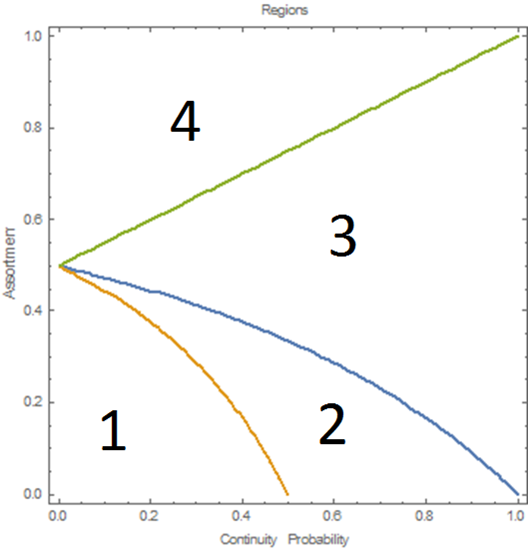
\includegraphics{regions}
\caption{Regions of Expected Behaviour}
\label{fig:regions}
\end{figure}

In Region I, ALLD is an equilibrium- determined by comparing the payoff of ALLD to a mutant that cooperates at least once. It is not the only equilibrium in the region, but equilibria strategies will play Defect against themselves and ALLD. In this region, cooperation is not expected; no cooperating strategy is an equilibrium.

In Region II, a variety of strategies are equilibria; for example, ALLD and TFT. So, both extremes of behaviour may be seen in a population under these circumstances. 

In Region III, there are again a variety of strategies that are equilibria, but ALLD and other complete defectors are no longer equilibria. Cooperative behaviour of varying types and degrees is expected to be common most of the time (equilibria can be escaped, for a short time).

In Region IV, ALLC is an equilibrium. All other equilibria always cooperate when playing against ALLC or themselves. Fully cooperative behaviour is expected to dominate. More regions are defined, but these are the ones of primary concern.

These general regions are expected to hold regardless of representation (I and II are particularly well defined, and not expected to vary).
The simulations \citet{van-veelen:PNAS:2012} conducted were of FSA with an unbounded number of states and half-memory (of unbounded length). The simulation is initialized with simple individuals: ALLD. Every member plays one other member of the population for a number of rounds determined stochastically, based on the continuation probability. With probability $r$ a member will play against an identical strategy. With probability $1-r$ a member will play against another player from the population. 

This payoff was used to calculate the probability for the individual to reproduce into the next generation. Stochastically, members of the population are selected for the new generation, so unfit individuals tend to be removed. 
During reproduction, mutation could also occur, resulting in new strategies. 

Results of the simulation were consistent with the analysis. 
A colourmap indicating the amount of cooperation in the simulation for varied continuation probabilities and assortment parameters was produced, with behaviour matching that predicted in each region. 
In general, both increased assortment and increased continuation probability increases cooperation (but there are exceptions). 

Indirect invasions are observed in the simulation \citep{garcia:PLoSOne:2012}. 
Indirect invasions are when a new strategy enters the population not by performing well against the currently dominant strategy, but by `springboarding' off another strategy. 
For example, consider that TFT is resistant to ALLD, and will only get exploited on the first move. 
ALLC is a neutral mutant of TFT (it plays against TFT the same way TFT plays against itself), and in a finite population of mostly TFT, ALLC can become more common by neutral drift. 
ALLD can exploit ALLC, and so when this neutral drift occurs, ALLD can use it to invade the population. 
This was summarised as: ``unconditional cooperation is therefore cooperation's worst enemy'' \citep{van-veelen:PNAS:2012}. 
Indirect invasions were observed establishing cooperative behaviour in a defecting population too. 

The results of the analysis should be valid regardless of representation. The simulation built upon previous work, investigating the interplay between reciprocity and population structure, and using unbounded rather than bounded FSAs allowing an infinite strategy space. 
However, the set of all possible strategies for the Prisoner's Dilemma is larger than this space. 

Other representations have their own strategy space. 
The choice of representation will exclude some, and enable some that were not possible in other representations. 
Representation also affects the chance of a strategy appearing, or the route by which it appears, since the mutation process may differ.
 
The model described in \citet{van-veelen:PNAS:2012} is the basis of my project. 
Both varied assortment and varied chance of a game continuing are modelled. 
Broad behaviour (such as whether strategies that always cooperate can dominate, or can be somewhat successful) can be predicted for ranges of assortment and continuation probability. This provides bounds for what behaviour is expected. 
Detailed behaviour can be discovered through simulation. 
The impact of variations in the simulation- such as changing how strategies are represented- can be compared quantitatively.
By using both assortment and continuation probability, conditions not explored in previous literature (with both assortment and reciprocity playing varied roles) can be investigated.

\chapter{Research Methods}
\label{chap:researchmethods}
In this section I will discuss the representation and mutation scheme I decided on (Pushdown Automata), the simulation I have created and how the analysis was carried out.

I focus on two mechanisms for the evolution of cooperation; direct reciprocity and assortment. 
These mechanisms can be simulated with differing lengths of games, and differing likelihood of strategies meeting other alike strategies. 
Other mechanisms, such as strategies having access to reputation (an opponents past with other strategies), require extra levels of complexity to enable this behaviour. 
The choice of these methods provides a simple starting point to investigate the interplay between mechanisms for cooperation. 

The Prisoner's Dilemma, as discussed in \ref{sec:prisoners} can be defined with a variety of payoffs so long as the heirarchy of payoffs is followed. 
To allow direct comparison to previous work (with no adjusting for Regions with a different payoff matrix), the same payoffs are used as \citet{van-veelen:PNAS:2012}. 
This is given in Table \ref{table:simpayoffs}.
 
\begin{table}[h]\centering
\captionsetup{justification=centering}
\begin{tabular}{|l|c|c|}
\hline
 & \bf{Cooperate} & \bf{Defect}\\
\hline
Cooperate & 2, \bf{2} & 0, \bf{3}\\
\hline
Defect & 3, \bf{0}  & 1, \bf{1} \\
\hline
\end{tabular}
\caption{Payoff matrix used in my simulations}
\label{table:simpayoffs}
\end{table}
%PAYOFFMARK
\section{Representation}
I have previously (Section \ref{sec:fsa} discussed Finite State Automata as a representations for strategies in repeated games. The representation I have used in my work is the Pushdown Automata, which can be thought of as an extension to Finite State Automata. 
%Other representations may be worth exploring, in regard to the question of how changing the strategy %space effects cooperation. These might include other models of computation such as a decision tree %model, or FSA with mixed strategies; with transitions with probabilities attached. 
%In this thesis, the focus is on Pushdown Automata. 
\subsection{Pushdown Automata}
Pushdown Automata can be briefly described as Finite State Automata that also interact with a stack memory. During each transition instead of simply reading from the input string (history of the game) and checking what transitions are valid, the machine (optionally)additionally checks what item is on the top of the stack. 
Whether a transition is valid is based on what is read, and what is on the top of the stack \citep[][pp 99 -- 122]{Sipser2006}. 

Each transition can $push$ a symbol from the stack alphabet to the stack. 

More formally, a PDA consists of:\\
1. A finite, set of states $S \neq  \emptyset$\\
2. An input alphabet, $\Sigma \neq  \emptyset$\\
3. A stack alphabet, $\Gamma$, containing a stack marker $Z_0$, the empty character which indicates no changes to the stack, and other stack symbols\\
4. A transition function $\delta : S \times \Sigma \time \Gamma \rightarrow \mathcal P(S \times \Gamma)$\\
5. A set of final/accepting states $F \subseteq S$ \\
6. The initial state $q_0 \in S$\\

Initially, the stack contains only the stack marker ($\Gamma_0=\{Z_0\}$).\\

A PDA is Non-Deterministic if more than one transition exists for any possible state and stack state.  If at most one transition exists for any possible state and stack state the Automaton is Deterministic. The language or set of strategies representable by a DPDA is a subset of strategies represented by PDA. The strategies represented by FSA are a subset of both. FSA can represent Regular strategies, DPDA can represent Deterministic Context-Free strategies, and PDA can represent Context-Free strategies.

\begin{figure}[h]
\centering
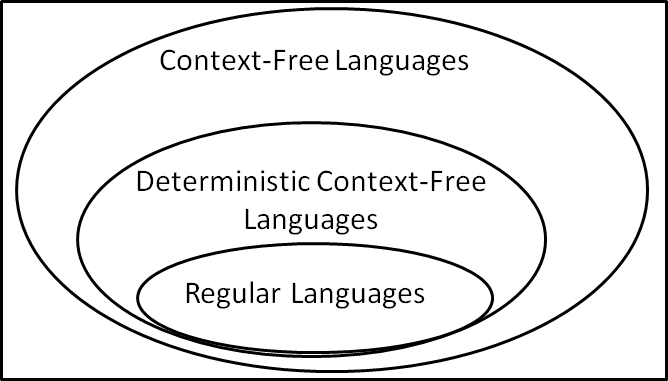
\includegraphics[width=0.7\textwidth]{languages}
\caption{Hierarchy of Strategy Spaces}
\label{fig:languages}
\end{figure}

Initially, I pursued simulating Non-Deterministic Pushdown Automata. 
This is a more complex task than simulating Deterministic Pushdown Automata, due to needing to maintain a set of valid configurations, since all possible paths must be followed to check if the input can leave the Automata in an accepting state. 
This results in more complicated software to create, and more computation needed to determine if one of the configurations is an accepting configuration. \\

I explored third party software for the task of implementing PDA; specifically \citet{JFLAP}. 
This was designed as a learning tool for Theory of Computation \cite{rodger2009increasing}, and for my purpose needed to be significantly modified. For example, current possible configurations would need to be maintained while waiting for the next input. The alternative already supported -- re-checking if the entirety of the current history instead of just iterating to the next item in the history -- was computationally expensive.  I made the decision to instead implement my own version of the simpler Deterministic Pushdown Automata, with the intention of expanding representations at a later stage. 
This reduced computation time, and simplified analysis. 

Figure \ref{fig:dpda} shows an example of a Deterministic Pushdown Automata. 
It should be familiar -- it is a variation of TFT. 
The character $\lambda$ is the empty symbol; no change is made to the stack when it is popped or pushed. Following the operation of this Automaton, we start on state $q0$. In all circumstances when a $C$ is read, and we are on state $q0$, $a$ is pushed to the stack. 
If $D$ is read, we do one of two things. If the stack is empty (indicted by \$ being on top of the stack), we move to state $q1$. 
If the stack is non empty, and so has a symbol from the alphabet on it, we $pop$ it and remain on $q0$. 
If we have transferred to $q1$ and read $C$, we $push$ $a$ and transfer back to the accepting/cooperating state. 
If we read $D$, we remain on the non-accepting state.

This example DPDA counts the number of times the opponent cooperates. 
If they have cooperated recently, it does not retaliate until defection moves outnumber cooperation moves. 
\begin{figure}[h]
\centering
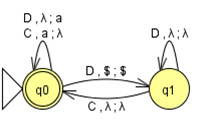
\includegraphics[scale=0.6]{pdatft}
\caption{Counting-TFT: A DPDA modelled off TFT, which counts Cooperation and Defection actions}
\label{fig:dpda}
\end{figure}
%\subsection{Deterministic Pushdown Automata}
The Automata used in my simulation are designed from a graph point of view. 
Each state in a DPDA is an object inside that DPDA, and each transition from a DPDA is an object inside that state. 
A DPDA is defined in the simulation by its initial state, its states (which include a boolean accepting/non-accepting marker) and its transitions (each belonging to a source state, and having a destination, $pop$ instruction, $push$ instruction and $read$ instruction). 

In my simulation, the strategies are given half-memory. 
This means they remember their opponents moves and not their own. 
So, a strategy cannot remember that its opponent defected in response to its own defection; the strategies that can appear are limited by this decision. 
The decision to use half-memory allows for direct comparison to previous work with FSA with half-memory \citep{van-veelen:PNAS:2012}, and simplifies analysis. 
The framework I have developed and will discuss further in this chapter will aid in extending this work to full-memory (remembering both the strategy and the strategies opponents histories) strategies. 

\subsection{Mutations}
As discussed in \ref{sec:mutation}, the mutation scheme is important. As long as it is a reasonable exploration of the strategy space we expect certain behaviour to hold, but much of the dynamics will be dependant on the mutation scheme chosen. Since I intend to extend work done with Finite State Automata, I have based my mutation scheme heavily on a mutation scheme for Finite State Automata \citep{van-veelen:PNAS:2012}.

The first mutation is the Add State mutation. A state is generated, which can be either an accepting state or a non-accepting state. Additionally, an outbound transitions is added with random $read$, $pop$, $push$ instructions and a random destination (with no bias towards 'nearby' states, or bias against the new state itself as the destination). One transition is rerouted with the new state as its destination, ensuring the new state is connected to the Automaton. 

Alternative mutation schemes could already be noted for just this first mechanism. 
The requirement that the new state be connected could be dropped- perhaps with justification to biological systems. Inactive information may exist in a genome. 
It could also be important- at some later stage it may be the subject of an advantageous mutation. 

The connected requirement is made because after mutations, the Automaton is pruned of disconnected states in order to address bloat \citep[][p 139]{koza}. 
Another alternative would be to not add any transitions to the new state- or to add an inbound transition rather than reroute an existing one. My method was chosen as it ensures connectedness and results in a smaller edit, when we define the size of an edit as the number of parameters changed. Four parameters must be added if a transition is inserted ($read$, $pop$, $push$, Destination), whereas the single re-routing is only one parameter change.

Removing a state is the second method of mutation. Outbound transitions from the state are deleted. 
Inbound states are randomly rerouted. When the re-routing results in an invalid automaton, the transition is deleted instead. Rerouting is chosen over deleting all related transition to minimize the size of the mutation. If the initial state is removed, another randomly chosen state is assigned as the initial state.

Adding a transition involves randomly selecting a source, destination, and $read$ $pop$ and $push$ instructions. All factors are uniformly selected, with the exception of only allowing a Stack interactions with a stack marker to both $pop$ and $push$; not one or the other. 

The remove transition mutation removes a transition. As a result, this may trigger more substantial changes to the Automaton. For example, it may disconnect the Automaton, making part unreachable and causing it to be pruned. 

Each parameter that a Transition contains can also change. It's destination state, $read$ condition, $pop$ condition and $push$ instruction can all be changed. These are selected randomly, with the exception of stack markers (with the $pop$ and $push$ condition as before). Transitions that would make the Automaton Non-Deterministic are simply not added, so the Automaton does not change on this mutation event in that case.

Finally, the accepting/non-accepting parameter of a state can be flipped.

This scheme can explore the entirety of the strategy space that can be represented by Deterministic Pushdown Automata which accept by final state, which includes all Finite State Automata.
\section{Simulation}
In my simulation, DPDA strategies compete with other DPDA strategies for survival and evolve \citep{fogel2006evolutionary}. 
The simulation uses a Wright-Fisher process. Figure \ref{fig:wright} gives an overview of this process. 
The population starts with all players using the strategy Always Defect. The always defect representation used is shown in Figure \ref{fig:alld}. In my output files, this would be given by ``S\#q0IT\#q0-q0vC.l-$>$l\&q0-q0vD.l-$>$l\&''. 
Each state is listed in the first section of this string, along with whether it is an inital $I$ and/or final $F$ state. $\#$ delimits sections. Transitions are given by {$stateFrom$-$stateTo$ }
Figure \ref{fig:wright} is started with a mixed population, to aid indicating how the process works. 
The population in simulations is of a fixed size $N$, and $N$ is even. 
Each player competes with a neighbour they are paired with, playing the repeated Prisoner's Dilemma, with the number of games they play dependent on the continuity probability $\delta$. 
Next, strategies reproduce, proportionally to payoffs. 

Strategies in an odd position reproduce by chance, based on fitness. 
In my example, A does well playing against the population, and is selected for the next generation. 
Not always however; since a lower fitness strategy still has a chance (a lower chance) of reproducing. 
Strategies in an even position reproduce by chance with probability $1-r$, where r is the assortment parameter, determining population structure.  This follows from \citet{van-veelen:PNAS:2012}, and guarantees that selection is not biased by this method of adding structure. 

Strategies in an even position have a probability $r$ of instead copying the neighbour strategy. 
This is the means by which assortment is added. 
Next, the population mutates. 
The mutation probability is low; ideally, an average of one mutant occurs per generation. 
If it were too high, analysis of whether a strategy can invade must consider a group of strategies entering at once rather than a single mutant. 

These steps repeat; with pairs competing again and so forth. 
The simulation is continued for a number of time steps that can be specified. 
Several parameters, including population size; the assortment parameter; the continuity probability; and how often the state of the simulation is recorded can be specified. 

A Wright-Fisher process is used as opposed to alternatives like a Moran process \citep{moran1962statistical} for less demanding computation. A Wright-Fisher process plays each player once against an opponent; a Moran process plays all players against all players. 

\begin{figure}[h]
\centering
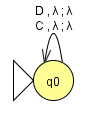
\includegraphics{alwaysDefect}
\caption{The initial strategy, Always Defect}
\label{fig:alld}
\end{figure}
\begin{figure}[h]
\centering
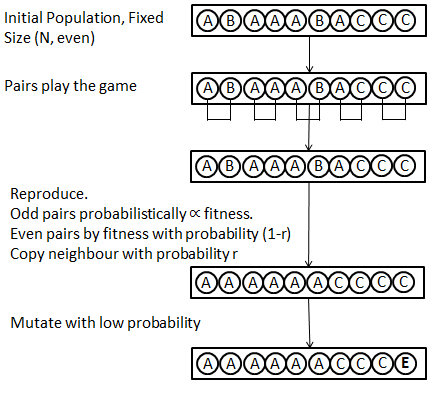
\includegraphics{wrightfischer}
\caption{Wright-Fischer Process}
\label{fig:wright}
\end{figure}
\pagebreak

My simulation extends simulations used for simulating the evolution of Finite State Automata \citep{van-veelen:PNAS:2012, jggit}. 
They accept a collection of parameters specifying the simulation, and output either a time series or an estimate of the payoff of the population. 
The time series contains the state of the population in specified generations. 
It reports the payoff of the population in that generation, the strategies present in the population, and the number of each strategy present. For example, a line of output may read:\\
``2023340,500.0,"Strategy : S\#q0FIT\#q0-q0vC.\$--$>$\$\&, Count : 250;"''\\
Meaning at generation 2023340 payoff was 500, and only one strategy was present (with a count of 250). 
This strategy is shown in Figure \ref{fig:grim}. 

\begin{figure}[h]
\centering
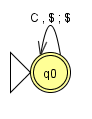
\includegraphics{grim}
\caption{The Grim Strategy}
\label{fig:grim}
\end{figure}
\pagebreak
Simulations were run with parameters as follows:
\lstinputlisting[frame=single]{Example.json}
Add state through to flip state specify mutation probabilities. 
In this case, all mutations are of similar probability; extra weight is given to transition changes as these transitions are small in comparison to others. 
They cause a less significant change to the Automaton than adding or removing a state or transition would.  
Other values could be argued for; a completely uniform probability, or a probability inversely proportional to the changes it causes, perhaps decided by the number of parameters that change. 

Reward, Temptation, Sucker and Punishment are parameters for the payoff matrix for the Prisoner's Dilemma. 
Population size, continuation probability $\delta$, assortment $r$ are also parameters -- with continuation probability and assortment the primary ones that are varied. 
The mutation probability per state gives the chance of a mutation occuring. In a population of 250 players playing a strategy with a single state, there will be an average of one mutation per generation with the probability given in this example (1/250). The mapping can be either Linear or Exponential (and is linear in simulations given in this thesis). 
Fitness is scored linearly in the first option, using an exponential function in the second. 
The intensity of selection is also selectable, and was set at 1.0 for simulations. 
If this is 0, there is no selection and likelihood of reproducing becomes entirely dependent on how populous a strategy is in the current generation (and an estimate of whether your mutation scheme is biasing defection or cooperation can be made). When this is 1.0, selection is strong. 

The mistake probability parameter is for adding noise-- where players make a choice, but perform the opposite choice. For most of the simulations presented, this was set to $0$ as the focus was on deterministic games. 
A generation limit, and how often to report is also specified. Additionally, the seed is recorded so simulations can be reproduced. This is also useful for running simulations with a smaller reporting interval, to see what is happening generation by generation in an interesting run. 

In my simulation, parameters for the Prisoner's Dilemma were R=2.0, T=3.0, S=0.0, P=1.0. 
All theoretical predictions are presented with this set of parameters. 
If the parameters change, the graph will change (but each region will still exist, and have the behaviour expected in that region). 

The Monash Campus Cluster \citep{cluster} was used for running simulations, due to the large amount of computation needed. 

\section{Analysis}
The primary output of the simulation is a time series. 
This includes the total payoff at each reported generation, the strategies present at each generation, and the number of each one of those strategies present. 
Several factors need to be examined. The first is the average payoff; is the population cooperative when continuity probability and assortment is set to a certain number. 
What strategies are common with theses parameters? 
The number of times each strategy is found over an entire run can be reported based on this time series, at which point the number of each strategy present when the strategy is common can be examined. Important factors to consider are how it enters the population, and how it exits if it does so. 

Two primary runs were conducted. 
The first run involved 882 simulations of time series; a 21$\times$21 grid of payoffs taken at data points spaced $0.05$ apart was taken (with $0.99$ instead of $1.0$ as the final point for the continuity parameter), twice. 
The second run involved 1640 simulations of times series, in order to find the payoffs as continuity probability and assortment are varied -- this time in a grid spaced $0.25$ apart (40$\times$41, as continuity parameter being 1 was excluded). 

These runs were processed using IPython notebook \citep{PER-GRA:2007}, finding the payoff for each time series, counting the strategies found in each run, and presenting the graph of payoff versus generation. 
The graphs of cooperation as continuity probability and assortment are varied were produced using gnuPlot \citep{Gnuplot_4.4}. 
The results of these simulations are discussed in the next chapter.

In addition to the time series simulations, I also created a function to compare the performance of strategies playing the Prisoner's Dilemma with varied continuity probability, assortment and noise. 
This does not evolve strategies, or simulate in an evolutionary environment. 
Instead it simply calculates expected payoff for each strategy. 
Based on the parameters, the game is repeatedly played and the results averaged. 
This gives an estimate, and not an exact value, of the payoff of each strategy. 
This is useful when the dynamics of three strategies needs to be investigated. 
The relative payoff for each strategy can be used with the replicator equation to estimate the rate of change for any proportion of each strategy; and so a phase diagram visualizing the dynamics can be plotted. 

\chapter{Results and Discussion}
\label{chap:results}
In this chapter, I present and discuss the overall cooperation observed with varied levels of assortment and continuation probability.  
The strategies present in points in each region of this graph-- individual time series-- are examined. Finally, new strategies that emerge and have not been previously reported in literature will be discussed. 
\section{Overall Cooperation}
\label{sec:overall}
Figure \ref{fig:cooperation} shows the cooperation observed in each region of the graph, for combinations of continuity parameter $\delta$ and assortment $r$. 
Cooperation is measured by the average payoff in the population; if all individuals are defecting all the time, the average payoff will be lowest (and equal to $P$). If all individuals are cooperating all the time, the average payoff will be highest (and equal to $R$). 
%Behaviour in each region will be discussed in more detail in Section \ref{sec:regions}.  
\begin{figure}[h]
\center
\includegraphics[width=0.6\textwidth]{{final_run.png}}
\caption{Cooperation observed}
\label{fig:cooperation}
\end{figure}
 
Figure \ref{fig:regions2}  \citep[adapted from][]{van-veelen:PNAS:2012} shows theoretical results describing how cooperation should vary across different regions of the parameter space (see Section \ref{sec:pnas}). 
Region I shows no cooperation. Region II shows a mixture of low cooperation with mostly defection.  Region III displays a mixture of mostly cooperation, with some defection. Region IV is fully cooperative. 
Notice the simulation results reported in Figure \ref{fig:cooperation} qualitatively match the theoretical prediction of Figure \ref{fig:regions2}. 
Differences, notably the larger levels of cooperation found above $r=0.5$, will be discussed in section \ref{sec:regions:3}. 

To assess the change in cooperative behaviour displayed in my simulations with previous work, I compare my graph of cooperation to that found by \citet{van-veelen:PNAS:2012}. 
Data from a separate simulation with sampled points matching points sampled from the previous work was used. 
The results of previous work  are shown in Figure \ref{fig:fsa} and the difference (measured as the relative error) is shown in Figure \ref{fig:difference}. 
In Region II, lighter/yellow areas of the difference graph indicate that my PDA simulation was up to 23\% less cooperative. 
In Region III, darker/purple areas of the difference graph indicate that my PDA simulation was up to 26\% more cooperative. 

\begin{figure}[h]
\center
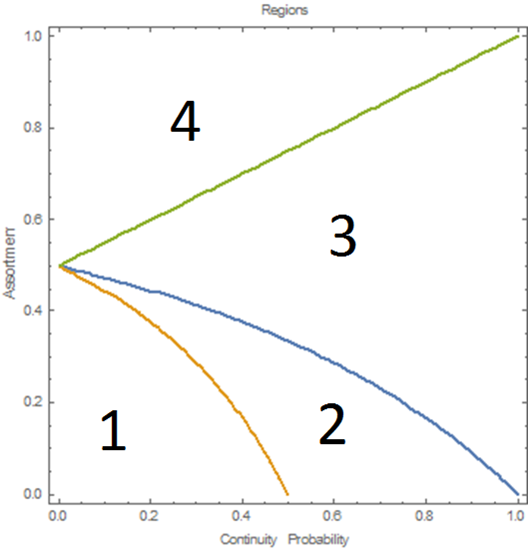
\includegraphics[width=0.45\textwidth]{regions}
\caption{Regions of Expected Behaviour}
\label{fig:regions2}
\end{figure}

\begin{figure}[h]
\subfloat[FSA results from \citet{van-veelen:PNAS:2012}\label{fig:fsa}]{
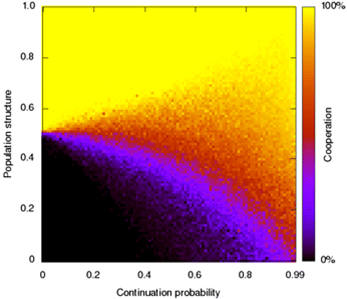
\includegraphics[width=0.45\textwidth]{fsa}}
\subfloat[Difference to FSA Paper\label{fig:difference}]{
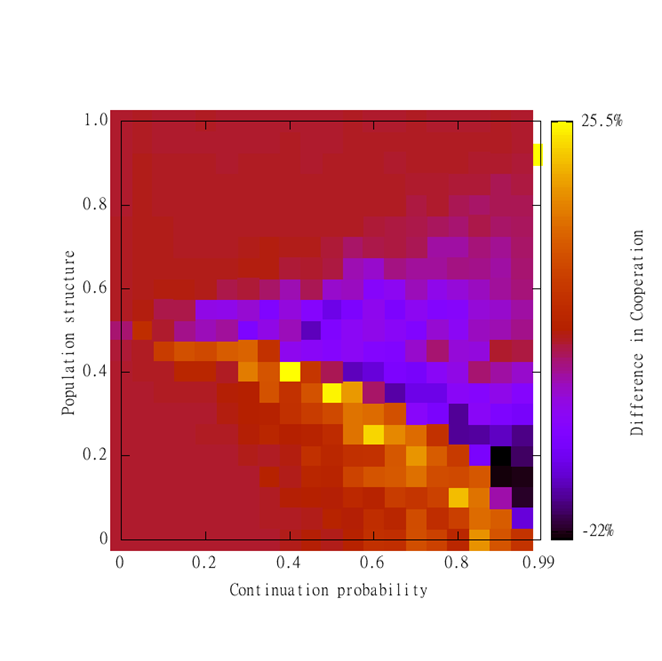
\includegraphics[width=0.45\textwidth]{cooperation}}
\caption{Comparison to FSA}
\label{fig:comparison}
\end{figure}
%\pagebreak

More cooperation was observed in Region III with my simulation, and less cooperation in Region II. 
The overall differences were minor, but may warrant further attention. 

\section{Behaviour in each Region}
\label{sec:regions}
The behaviour in each region can be predicted qualitatively, without assuming any specific representation (see Section \ref{sec:pnas}). 
The cooperation over time for each part of the graph -- for each combination of assortment and continuation probability, will be examined. 

Note that the Regions shown are for the game used in the simulation. 
If parameters are changed, the regions in the graph will shift (but the behaviour will still be qualitatively defined). 

\subsection{Region I: Small $\delta$, Small $r$}
In Region I, full defection is the only equilibrium. 
No strategy that plays cooperatively is expected to be successful. 
Time series of this region are given in Figures \ref{fig:first1} to \ref{fig:last1}. 
The x-axis corresponds to the generation, and the y-axis corresponds to the total population payoff. 
Larger payoffs indicate more cooperation. 

\begin{figure}[h!]
\centering
\includegraphics[width=0.9\textwidth]{{dataset1_0.0_0.0}.png}
\caption{Time series when $\delta=0.0$, $r=0.0$}
\label{fig:first1}
\end{figure}
\begin{figure}[h!]
\centering
\includegraphics[width=0.9\textwidth]{{dataset1_0.2_0.2}.png}
\caption{Time series when $\delta=0.2$, $r=0.2$}
\label{fig:1-0.2-0.2}
\end{figure}
\begin{figure}[h!]
\centering
\includegraphics[width=0.9\textwidth]{{dataset1_0.0_0.4}.png}
\caption{Time series when $\delta=0.0$, $r=0.4$}
\label{fig:last1}
\end{figure}
In these time series, cooperation does not survive long in the population, and do not come to be the most common strategy. 
Closer to the border of this region (with larger $r$, Figure \ref{fig:last1}), the environment becomes noisier. 
The qualitative prediction given by \citet{van-veelen:PNAS:2012} holds close to the border, but selection against any cooperator is more extreme in regions close to $r=0$,$\delta=0$. 

On the upper border, towards greater assortment, (outside Region I), cyclic behaviour is observed (Figure \ref{fig:cycles1}, with time range limited to better visualize cycles). 
On the right border, towards greater continuation probability, results are more noisy but still overwhelms any cooperative strategies. 
\begin{figure}[h!]
\centering
\includegraphics[width=0.9\textwidth]{{dataset1_0.0_0.5}.png}
\caption{Time series when $\delta=0.0$, $r=0.5$}
\label{fig:cycles1}
\end{figure}

In Region I, strategies that are mutually defecting are most common. 
No strategy in the top 25 most common strategies found in these regions in my simulation has a cooperating states; all are variants of Always Defect. 
This is the expected behaviour in this region of the parameter space. 
\subsection{Region II: Small $r$}
In Region II, some cooperators and some defectors are equilibria. 
Essentially, anything goes in this region. 

Figures \ref{fig:2-0.5-0.2} and \ref{fig:2-0.5-0.3}, and Figures \ref{fig:2-0.7-0.1} and \ref{fig:2-0.7-0.3} show the increase in cooperative behaviour as the combination of continuity probability and assortment increases, making the situation considered closer to the border with Region III. 

In these time series, except in the case of Figure \ref{fig:2-0.7-0.3} the most common strategies are mutually defecting.
In Figure \ref{fig:2-0.7-0.3}, Grim and Defect are most common, making up 64\% and 36\% of the proportion of the top 20 strategies. 
These strategies are all representable by FSA. 
\begin{figure}[h!]
\centering
\includegraphics[width=0.8\textwidth]{{dataset2_0.5_0.2}.png}
\caption{Time series when $\delta=0.5$, $r=0.2$}
\label{fig:2-0.5-0.2}
\end{figure}
\begin{figure}[h!]
\centering
\includegraphics[width=0.8\textwidth]{{dataset2_0.5_0.3}.png}
\caption{Time series when $\delta=0.5$, $r=0.3$}
\label{fig:2-0.5-0.3}
\end{figure}
\begin{figure}[h!]
\centering
\includegraphics[width=0.8\textwidth]{{dataset2_0.7_0.1}.png}
\caption{Time series when $\delta=0.7$, $r=0.1$}
\label{fig:2-0.7-0.1}
\end{figure}
\begin{figure}[h!]
\centering
\includegraphics[width=0.8\textwidth]{{dataset2_0.7_0.3}.png}
\caption{Time series when $\delta=0.7$, $r=0.3$}
\label{fig:2-0.7-0.3}
\end{figure}

\begin{figure}[h!]
\centering
\includegraphics{{handshakeparent}.png}
\caption{A Strategy with a Handshake}
\label{fig:handshakeparent}
\end{figure}

\begin{figure}[h!]
\centering
\includegraphics{{handshakechild}.png}
\caption{Mutant of Figure \ref{fig:handshakeparent}}
\label{fig:handshakechild}
\end{figure}

In Figure \ref{fig:2-0.7-0.3} a strategy that defects twice, then cooperates against itself appears. 
This strategy is given in Figure \ref{fig:handshakeparent} 
Before this strategy appears, the population is a combination of Always Defect variants. 
With non-zero assortment ($r=0.3$) this strategy is more likely to encounter itself. 
So, when it appears, its lower payoff against Always Defect is offset by encounters with itself. 
Eventually, a new strategy (child) that is neutral to it drifts in. 
The strategy performs the `handshake' of two defects playing itself (or its ancestor with the same behaviour). 
However, Grim Trigger, which cooperates until a defection happens, then never cooperates again eventually takes over. 
The ancestor strategy would beat Grim-- it exploits it in the first move, and thereafter mutual defection occurs. 
The child strategy however cooperates if the opponents first move is cooperation, then cooperates again if it follows up with a defection.
So, the new strategy wins the first move, but loses the next two. 
Thereafter defection is mutual. 
A neutral mutant of the ancestor provided the means for Grim Trigger to invade-- an indirect invasion. 

Figure \ref{fig:handshake} shows the approximate dynamics of this invasion. 
This was estimated by using the strategy comparison feature of my program; payoffs are estimated playing each strategy. 
Dynamo \citep{dynamo} uses the replicator equation to estimate evolutionary dynamics. 
In reality, the bottom two strategies are neutral to each other, where the graph suggests drift towards either strategy, depending on starting conditions. 

It does capture the invasion however; initially the population is Handshake. Handshake neutrally to Handshake-Child. Once Handshake-Child is the majority strategy, Grim is selected for (and invades once it appears via mutation). 
\begin{figure}[h!]
\centering
\includegraphics[width=0.6\textwidth]{{handshakeinvasion}.png}
\caption{Dynamics of Handshake, Handshake-Child and Grim: An indirect invasion}
\label{fig:handshake}
\end{figure}

\begin{figure}[h!]
\centering
\includegraphics[width=0.8\textwidth]{{dataset2_0.95_0.0}.png}
\caption{Time series when $\delta=0.95$, $r=0.0$}
\label{fig:2-0.95-0.0}
\end{figure}

\begin{figure}[h!]
\centering
\includegraphics[width=0.8\textwidth]{{dataset2_0.99_0.00}.png}
\caption{Time series when $\delta=0.99$, $r=0.0$}
\label{fig:2-0.99-0.0}
\end{figure}

Figure \ref{fig:2-0.95-0.0} and \ref{fig:2-0.99-0.0} show the case of high continuity probability with no assortment. 
As continuity probability increases, cooperation becomes more frequent. 
In this region, both Grim, Always Defect and Always Cooperate appear. 
Grim appears with highest frequency (94\% of the proportion of the 10 most frequent strategies). 

A Non-Regular strategy appears regularly in this region. 
This is shown in Figure \ref{fig:grudge}, and I have called Counting Grudge. 
It pushes a symbol to the stack whenever the opponent cooperates. 
It pulls from the stack whenever the opponent defects. 
If at any point the number of defection actions outnumber cooperation actions, it stops cooperating. 
There is no valid transition for an empty stack and reading a $D$ action, so any future moves are not in the language the DPDA describes; the strategy will always defect from this point. 
Counting Grudge only makes up 3\% of the top 10 most frequent strategies at this point. 
However, it appears in other simulations in Region II and Region III too. 
It will prove relevant in Section \ref{sec:noise}, where I will discuss when DPDA may be advantageous strategies.
\begin{figure}[h!]
\centering
\includegraphics[scale=0.5]{{grudge}.png}
\caption{Counting Grudge: A DPDA Strategy that counts Cooperation and Defection actions}
\label{fig:grudge}
\end{figure}

\subsection{Region III: Varied $\delta$, Varied $r$}
\label{sec:regions:3}
In Region III, full mutual defection is not an equilibria. 
Non-zero cooperation is expected throughout this region, though not necessarily full cooperators. 
\begin{figure}[h!]
\centering
\includegraphics[width=0.8\textwidth]{{dataset3_0.4_0.45}.png}
\caption{Time series when $\delta=0.4$, $r=0.45$}
\label{fig:3-0.4-0.45}
\end{figure}
\begin{figure}[h!]
\centering
\includegraphics[width=0.8\textwidth]{{dataset3_0.6_0.4}.png}
\caption{Time series when $\delta=0.6$, $r=0.4$}
\label{fig:3-0.6-0.4}
\end{figure}
\begin{figure}[h!]
\centering
\includegraphics[width=0.8\textwidth]{{dataset3_0.6_0.5}.png}
\caption{Time series when $\delta=0.6$, $r=0.5$}
\label{fig:3-0.6-0.5}
\end{figure}
\begin{figure}[h!]
\centering
\includegraphics[width=0.8\textwidth]{{dataset3_0.6_0.7}.png}
\caption{Time series when $\delta=0.6$, $r=0.7$}
\label{fig:3-0.6-0.7}
\end{figure}
\begin{figure}[h!]
\centering
\includegraphics[width=0.8\textwidth]{{dataset3_0.95_0.2}.png}
\caption{Time series when $\delta=0.95$, $r=0.2$}
\label{fig:3-0.95-0.2}
\end{figure}

Below $r=0.5$, expected behaviour is observed. 
Cycles between cooperation and defection occur, with cooperation being more prevalent as $\delta$ and/or $r$ increase. 
In Figure \ref{fig:3-0.95-0.2} the previously discussed two-defection handshake, then cooperate strategy reappears when the payoff of the population is approximately 430 for over 100,000 generations. 

In this region, Grim Trigger is the most common strategy. 
Always Cooperate and Counting Grudge also appear. 
Counting Grudge appears when continutity probability is high. 
One difference from previous FSA simulations is the Region where $r>0.5$. 
Full cooperation is observed, where defectors are predicted to invade with limited success. 

When $\delta$ is small, some of Region III does have less than full cooperation. 
As $\delta$ increases, full cooperation is seen. 
The rate at which Grim appears with my simulations mutation scheme explains this behaviour. 
For high $\delta$, Grim is able to resist defectors. 
It plays well against itself, and when many games are played the payoff is near mutual defection for both parties -- only on the first round of an interaction does Grim do worse than a defector. 
The population can drift away from Grim to other mutually cooperative strategies, like Always Cooperate. 
But, the small number of mutations required for Grim to reappear make invasions by strategies that exploit highly cooperative strategies short lived; a strategy is likely to mutate to Grim, and Grim is likely to invade if that defector gains any ground.

\begin{figure}[h!]
\centering
\includegraphics[width=0.8\textwidth]{{dataset3_0.4_0.6}.png}
\caption{Time series when $\delta=0.4$, $r=0.6$}
\label{fig:3-0.4-0.6}
\end{figure}

\begin{figure}[h!]
\centering
\includegraphics[width=0.8\textwidth]{{dataset3_0.7_0.6}.png}
\caption{Time series when $\delta=0.7$, $r=0.6$}
\label{fig:3-0.7-0.6}
\end{figure}
\subsection{Region IV: Varied $\delta$, Large $r$}
In Region IV, mutual cooperators are the only equilibrium strategies. 
In this region, Grim is again common. 
When continuity probability is low, ($\delta<0.5$), and a single round is likely, Automata with a single accepting state and no transitions -- which cooperate on the first round, and defect on later rounds which are unlikely to occur -- also appear. 
Mutual defection is observed, as seen in Figures \ref{fig:4-0.2-0.6} and \ref{fig:4-0.0-0.9}.
\begin{figure}[h!]
\centering
\includegraphics[width=0.8\textwidth]{{dataset4_0.2_0.6}.png}
\caption{Time series when $\delta=0.2$, $r=0.6$}
\label{fig:4-0.2-0.6}
\end{figure}
\begin{figure}[h!]
\centering
\includegraphics[width=0.8\textwidth]{{dataset4_0.0_0.9}.png}
\caption{Time series when $\delta=0.0$, $r=0.9$}
\label{fig:4-0.0-0.9}
\end{figure}
Data points closer to the boundary with Region III are noisier than those in the center of the region, but mutual cooperation remains the overwhelmingly most frequent strategy used. 
\section{Successful DPDA Strategies}
\label{sec:dpdaresults}
In Region II and III, a DPDA was seen amongst the most common strategies. 
It was not the most successful strategy; it is neutral to Grim and any mutually cooperative strategy. 
Intuitively, we may expect DPDA to do relatively well in a noisy environment. 
In a noisy environment, actions chosen by players are occasionaly reversed. 
In this environment, Grim would immediately retaliate to defection, that could have been performed accidentally. 
Counting Grudge will not retaliate so quickly once cooperation is established. 
In this section, I add noise to the simulation, and highlight where this DPDA becomes a successful strategy. 
\subsection{Games with Noise}
\label{sec:noise}
The simulation was ran with noise of 0.01 and 0.05, all other parameters were held the same. 
With noise 0.01, 1 percent of moves are inverted; the strategy cooperates when they meant to defect and vice-versa. 
In this case, Counting Grudge makes up 25\% of the strategies of the top ten most common. 

Does Counting Grudge do a good job against other strategies I expect in this region. 
I pitted it against Tit-For-Tat (a strategy that did not appear commonly in my simulation, due to mutation distance) and Always Cooperate, instead of operating in an simulated evolutionary environment, I played them against each other in the environment and estimated the expected payoff against each other. 
The expected payoff is then used to make a simplex of the dynamics; with the changing population estimated using the replicator equations. 
The result is shown in Figure \ref{fig:noisesimplex}. 
A stable point exists at all 3 points, but the interior of the phase diagram points to Counting Grudge. 

\begin{figure}[h!]
\centering
\includegraphics[width=0.5\textwidth]{{Noise001}.png}
\caption{Counting Grudge playing TFT and ALLC in an environment with 1\% noise}
\label{fig:noisesimplex}
\end{figure}

The advantage of a stack in this case is the ability to do simple counting, without needing to have extra states. The number of cooperation -- and so if the opponent has been overall cooperative -- can be accomplished with a single state, two transitions and a stack. 
Whereas Tit-For-Tat retaliates against a defection immediately, Counting Grudge will wait until defections outnumber cooperative moves. 
FSA can accomplish this; but again, require extra states for each level of `tolerance'. 
In a noisy environment, it can pay to be forgiving of mistakes. 

Counting Grudge is still exploitable; for example, a strategy that cooperates a few times to establish some `leeway' -- some symbols on the stack. 
The strategy can then alternate cooperate and defect fairly safely; it is unlikely that enough mistakes will be made (due to noise) that the number of defection moves outnumber cooperative moves. 
So, for every second move this strategy gets the highest payoff possible for a round. 

Successful DPDA do appear; one notable example was discussed. 
Further analysis of noisy environments may yield interesting results.
\chapter{Conclusions}
\label{chap:conclusions}
I investigated the evolution of strategies representable by Deterministic Pushdown Automata. 
My simulation allowed for varied continuity probability and assortment parameters, and reported behaviour that results and the strategies that appear. In this chapter, I will discuss the results in regards to my research questions.
\section{Effect on Cooperation}
In Section \ref{sec:overall} I discussed the observed differences in the amount of cooperation in each region to previous results. 
In Region II, the FSA simulation found higher cooperation \citep{van-veelen:PNAS:2012}. 
In Region III, my DPDA simulation found higher cooperation. 
The non-appearance of DPDA in my simulation in Region II suggests that these differences are a result of the mutation scheme used for each model. 
My simulation explored the strategy space differently, so different strategies with different levels of cooperation evolved. 
\section{Comparison to Theory}
Section \ref{sec:regions} examined the Time Series in each region. 
My simulation gave results that did not violate the expected outcomes. 
However, some differences in what you might expect (but not differences from the limits to behaviour \citep{van-veelen:PNAS:2012} defined) did appear. 

When $r>0.5$ and $\delta>0.5$, so both assortment and continuity probability are high, no partially defecting strategies are successful. 
This appears to be a result of the mutation scheme used; Grim entered the population too quickly for non-cooperative strategies to survive for long.
\section{The Evolution of Successful Non-Regular Strategies}
\label{sec:dpda}
Non-Regular strategies, evolved in my simulation. One which appeared with high frequency when continuity was high, was Counting Grudge. 
However, its success was limited. 
Being neutral to Always Cooperate and Grim, it does not have an advantage over these in an environment without defectors or noise. 
Adding noise, I showed that Counting Grudge can be more successful than some other strategies expected to appear in regions of the graph with cooperation present. 
\section{Future Work}
I would like to extend the work I have conducted this year to further examine Non-Regular strategies in noisy environments. 
The strategies that can be represented by Deterministic Pushdown Automata could be examined more thoroughly with theory, including in noisy environments. 

Other strategy representations could be explored, such as decision trees, or Non-Deterministic Pushdown Automata. 
A simple extension to my work would be to use Full-Memory Deterministic Pushdown Automata.
\appendix % all \chapter{..} commands after this will generate appendices

\chapter{Simulation}
Here I will have a brief readme.
\section{Source Code}
\label{app:code}
Here I will detail how to get the source code of my program. 
\section{Design}
Here I will add a class diagram
\section{Public Release}
I will also state where I am going to post my code on git.

%%%%%%%%%%%%%%%%%%%%%%%%%%%%%%%%%%%%%%%%%%%%%%%%%%%%%%%%%%%%%%%%%%%%%%%%%%%%%%
%%
%% Back matter 
%%

%\backmatter						% start the thesis back matter
%\begin{thesisauthorvita}
%\begin{spacing}{1}
%Publications arising from this thesis include:
%\begin{description}
%\item[Author, A.\ and Bloggs, J.\ (2002),]
%A really catchy title. In \emph{The 31st International Conference
%on Non-specific Computing.} Capital City, Country.
%\item[Bloggs, J.\ and Author , A. (2002),]
%A very much longer and significantly less catchy title. in \emph {Workshop on
%A Research Area}. Springfield, USA.
%\end{description}
%\end{spacing}
%\end{thesisauthorvita}

\bibliographystyle{dcu} % A good style to use with the Harvard package
\bibliography{../bibliography}

%\chapter{Last Thing} % Appendices after the \backmatter command do not
						% get a letter
%This sort of appendix has no letter. 


\end{document}
